\chapter{Experiments with Black-Scholes dynamics}

The Black--Scholes framework rests on: (i) a frictionless, arbitrage-free market with continuous trading and no transaction costs; (ii) a risky asset $S_t$ with \emph{constant} instantaneous drift $\mu$ and volatility $\sigma>0$; (iii) a constant risk-free rate $r$; (iv) log-normally distributed asset prices, driven by a single standard Brownian motion $W_t$ under the physical measure $\mathbb{P}$; and (v) no dividends, jumps, or stochastic volatility.

Under $\mathbb{P}$, the asset price follows a geometric Brownian motion (GBM):
\begin{equation}
dS_t = \mu S_t\, dt + \sigma S_t\, dW_t, \qquad S_0 > 0.
\end{equation}
Under the risk-neutral measure $\mathbb{Q}$, obtained via Girsanov's theorem with market price of risk $\lambda = (\mu-r)/\sigma$, the drift is replaced by $r$:
\begin{equation}
dS_t = r S_t\, dt + \sigma S_t\, dW_t^{\mathbb{Q}}.
\end{equation}


Applying It\^o's lemma to $\ln S_t$ yields the exact solution
\begin{equation}
S_t = S_0 \exp\left[\left(r - \tfrac{1}{2}\sigma^2\right)t + \sigma W_t^{\mathbb{Q}}\right],
\end{equation}
so that $\ln S_t \mid S_0 \sim \mathcal{N}\!\left(\ln S_0 + (r-\tfrac12\sigma^2)t,\; \sigma^2 t\right)$: log-returns are Gaussian and i.i.d.\ over disjoint intervals, and $S_t$ is log-normal.


Sample paths are continuous (no jumps), Markovian, and self-similar in the sense $S_{t+\Delta}/S_t \stackrel{d}{=} S_\Delta/S_0$ with instantaneous variance constant.


\section{Data and Training procedure}

For each trajectory $j = 1, ..., J$ we define 
the SDE of the log-price $X_t^j$ to be modelled using the Black-Scholes framework where the only source of uncertainty is given by the Brownian motion $W_t$:
\begin{equation}
    \label{log-price SDE}
    \begin{aligned}
       &dX_t^j = -\frac{1}{2}\sigma_j^2 dt + \sigma_j dW_t\\
         &\text{with } X_0^j = \log(S_0^j)
    \end{aligned}
    \end{equation} 

Where $S_0^j$ is the raw price at time $0$ of trajectory $j$, $\sigma_j$ is the volatility of trajectory $j$ and $W_t$ is a standard Brownian motion.
In this setting we are emulating the scenario of working under the risk-neutral measure $\mathbb{Q}$ with zero interest rate and zero dividend yield.\\
$X_0^j$ and $\sigma_j$ are randomly sampled for each trajectory such that 
$X_0^j \in [-1, 1]$ and $\sigma_j \in (0.0, 1.2]$.\\

In this context our condition $c_j$ for a general data observation $j$ is given by
a vector containing the trajectory $c_j=[X_0^j, X_{dt}^j, X_{2dt}^j, ..., X_{Ndt}^j]$.

 The SDE is discretized over a uniform time space $N dt = T$ obtaining the following form
 adopted for the simulation of the trajectories:
 \begin{equation}
    \label{eq: discretized_SDE}
    X_{t+dt}^j = X_t^j -\frac{1}{2}\sigma_j^2 dt + \sigma_j \sqrt{dt} Z_t
 \end{equation}
 Where $Z_t \sim \mathcal{N}(0,1)$.\\
The procedure to build the condition data matrix $C$ is summarized in Algorithm \ref{alg:y condition}.

\begin{algorithm}[H]
\caption{Algorithm for the condition data matrix $C$ creation}
\label{alg:y condition}
\begin{algorithmic}[1]

\STATE Define the number of simulation $J$.
\STATE Initialize an empty data matrix $C$ of shape $J\times N$.
\STATE Set iteration counter $j \leftarrow 0$.
\REPEAT
    \STATE Randomly sample $\sigma_j \in (0.1, 1.2)$ with $X_0^j = 0.0$.
    \STATE Evolve $X_t^j$ based on the discretized SDE for $0, dt, ..., Ndt$ steps.
    \STATE Store the trajectory $[X_0^j, X_{dt}^j, X_{2dt}^j, ..., X_{Ndt}^j]$ in the $j$-th row of $C$.
    \STATE Increment counter $j \leftarrow j + 1$.
\UNTIL{$j = J$}
\RETURN $C$
\end{algorithmic}
\end{algorithm}


Since the ForGAN architecture is adopted, which is trained to generate the next value of the trajectory,
the output data $X$ is a $J \times 1$ vector where each element is the $n$-th step ahead value of the trajectory, 
so the output is a single value and not a probability distribution during training time. 
In this case, the target output data matrix $X$ is computed by evolving each trajectory for the $\tau$-th step using the discretized SDE 
described in  \ref{eq: discretized_SDE} and storing the resulting value in the $j$-th position of $X$.\\

Now that the training data are defined the ForGAN model can be trained by using both the classical BCE loss, using algorithm \ref{alg: cgan}
and the Wasserstein loss with gradient penalty using algorithm \ref{alg:cwgan_gp}.
 




After the training phase, the ForGAN is able to generate the future distribution by repeatedly sampling the next value of the trajectory by using different noise realizations, as described in \ref{alg: forgan-inference}.\\
At the end of the condition trajectory, so at time $T=N dt$, we have the following information: the final log-price $X_{Ndt}^j$ of each trajectory $j$ and the corresponding volatility $\sigma_j$.
The goal of the Conditional GAN is to learn the distribution of final values of the stochastic process at next time horizon $T + \tau$. 
A theoretical closed form can be used as ground truth. It is given by a normal distribution:
\begin{equation}
    \begin{aligned}
    X_{Ndt + \tau}^j & \quad \sim \quad \mathcal{N}(X_{Ndt}^j - \frac{1}{2}\sigma_j^2 \Delta t, \sigma_j \sqrt{\Delta t})\\
    \text{where } &\Delta t = dt \times \tau \text{ with $\tau$ the number of days ahead. }
    \end{aligned}
\end{equation}


In order to provide a comparison between the proposed ForGAN architectures and 
the theoretical solution of the GBM processes, the target distribution $x$ of the next value $c_{T + \tau}$ of the process is computed by using the Monte Carlo algorithm described in \ref{alg:mc_terminal_dist}.
This is required to properly evaluate the model's performance because since the ForGAN model provides the distribution of the next value by repeated sampling, the vector of those samplings needs to be converted into a probability distribution. 
So, it is required a uniform way to compute the bins values used to build the empirical distribution.\\
In fact, after the Monte Carlo simulations are performed, the resulting terminal values are used to build the empirical distribution of the next value $c_{T + \tau}$ by using $\sqrt{n_{mc\_simulations}}$ as rule of thumb to compute the optimal number of bins for the histogram. 
The same bins are then used to compute the empirical distribution of the generated samples from the ForGAN model.\\
Alternatively, the Freedman-Diaconis rule can be used \cite{forgan:freedman_bins} to compute the optimal bin width for complex target distributions.
The Freedman-Diaconis rule provides a robust statistical method for determining optimal histogram bin width by minimizing the integrated mean squared error. 
Unlike methods sensitive to outliers, it utilizes the interquartile range (IQR) to account for data variability. 
The bin width $h$ is calculated as:$h = 2 \cdot \frac{\text{IQR}(x)}{\sqrt[3]{n}}$ where $n$ represents the number of observations.
By prioritizing the spread of the central 50\% of the distribution, 
the algorithm ensures that the resulting binning structure accurately reflects the underlying density of the empirical data without over-smoothing or producing noise-induced artifacts.\\

The algorithm to compute the theoretical distribution $p(x|c)$ given Monte Carlo simulations and the ForGAN's generated distribution are as follows:
\begin{algorithm}[H]
\caption{Monte Carlo generation of terminal distributions}
\label{alg:mc_terminal_dist}
\begin{algorithmic}[1]
\REQUIRE Number of trajectories $J$, steps ahead $N$, and MC simulations $K$, final values from which to compute the distribution $\mathbf{C}_T \in \mathbb{R}^J$, drift $\boldsymbol{\mu} \in \mathbb{R}^J$, volatility $\boldsymbol{\sigma} \in \mathbb{R}^J$, and time increment $ dt$.
\STATE \COMMENT{Generate random standard normal shocks for all trajectory $j$ and simulation $k$}
\STATE $\mathbf{Z} \leftarrow \text{Tensor}(J, K)$ where $Z_{j, k} \sim \mathcal{N}(0,1)$
\STATE $\Delta t = dt * N$
\FOR{each trajectory $j \in \{1, \dots, J\}$}
    \STATE \COMMENT{Calculate the deterministic drift component per step}
    \STATE $\mathbf{d_j} \leftarrow (\boldsymbol{\mu_j} - 0.5 \boldsymbol{\sigma_j}^2) \Delta t$ 
    \STATE \COMMENT{Compute stochastic shocks for simulation $k$}
    \STATE $\mathbf{S}_{k}^j \leftarrow \sigma_j \cdot Z_{j, k} \cdot \sqrt{\Delta t}$
    \STATE \COMMENT{Calculate increments for each simulation $k$}
    \STATE $\boldsymbol{\delta}_{k}^j \leftarrow d_j + S_{k}^j$ 
    \FOR{each simulation $k \in \{1, \dots, K\}$}
        \STATE $X_{k}^j \leftarrow C_{T,j} + \delta_{k}^j$
    \ENDFOR
\ENDFOR
\STATE $\mathbf{X} \leftarrow \text{Matrix}(J, K)$
\STATE Compute $\mathbf{D} \leftarrow \quad$ the normalized histogram of $\mathbf{X}$ to estimate the empirical distribution for each trajectory $j$ using $n_{bins} = \sqrt{K}$ or alternatively the method in \cite{forgan:freedman_bins}.
\RETURN $\mathbf{D}$, $\mathbf{bins}$ \COMMENT{The empirical probability distributions for each trajectory}
\end{algorithmic}
\end{algorithm}






\begin{algorithm}[H]
\caption{ForGAN distribution inference}
\label{alg: forgan-inference}
\begin{algorithmic}[1]
\REQUIRE Trained generator parameters $\theta_G$, conditioning history $c_j$, number of samples $V$
\STATE Initialize an empty list $\mathcal{S} \leftarrow \emptyset$ to store generated samples.
\FOR{$i = 1$ \TO $V$}
    \STATE Sample latent noise $z^{(i)} \sim p_z$ \COMMENT{Independent noise draw, same $c_t$}
    \STATE $\hat{x}_{t+h}^{(i)} \leftarrow G(z^{(i)}, c_j)$ \COMMENT{Generate candidate forecast}
    \STATE $\mathcal{S} \leftarrow \mathcal{S} \cup \{\hat{x}_{t+h}^{(i)}\}$
\ENDFOR
\RETURN $\mathcal{S}$ \COMMENT{ list of generated samples for empirical distribution of trajectory $j$}
\end{algorithmic}
\end{algorithm}

After having obtained $D$ from \ref{alg:mc_terminal_dist} and having computed the ForGAN inferred distribution by normalizing the histogram of $\mathcal{S}$ obtained from \ref{alg: forgan-inference} by using the same $bins$ from \ref{alg:mc_terminal_dist},
the two distributions can be compared by using all the metrics described in \ref{sec:performance_metrics} like Jensen-Shannon divergence, Wasserstein distance, Total Variation distance and statistical tests like the Kolmogorov-Smirnov test.


\subsection{ForGAN simplified task}
In the following section a simplified version of the problem is discussed.
In particular, here the condition vector is given by just trajectories obtained from the same volatility parameter $\sigma = 0.5$,
which will be constant for all 
the trajectories.
The goal of this experiment is to understand if the proposed ForGAN architecture is able to capture the variance and mean of the target distribution when the volatility is fixed for all trajectories.

Below are presented the architecture and metrics results for the simple ForGAN architecture:
\begin{table}[H] 
\centering
\caption{ForGAN Architecture and Hyperparameters Summary}
\label{tab:forgan_debug_architecture}
\begin{tabular}{lll}
\hline
\textbf{Parameter}         & \textbf{Generator}            & \textbf{Critic (Discriminator)} \\ \hline
Input Dimension            & 32 (Latent) + 2 (Cond.)       & 1 (Data) + 2 (Cond.)            \\
Hidden Layers              & [64, 128, 64]                 & [64, 128, 128, 64, 32]          \\
Output Dimension           & 1                             & 1                               \\
Activation Function        & Leaky ReLU                    & Leaky ReLU                      \\
Normalization              & BatchNormalization            & None                            \\
Dropout                    & 0.0                           & 0.0                             \\
\multicolumn{3}{c}{\textbf{Global Training Settings}}                                     \\ \hline
Max Epochs                 & \multicolumn{2}{l}{100}                                       \\
\end{tabular}
\end{table}

\begin{table}[h]
\centering
\begin{tabular}{l c}
\hline
\textbf{Metric} & \textbf{Value} \\
\hline
\label{tab:forgan_debug_results}
KS Test Acceptance (\%) & 1.0000 \\
JS Distance & 0.1757 \\
Hellinger Distance & 0.1520 \\
TV Distance & 0.1440 \\
EMD Distance & 0.0049 \\
\hline
\end{tabular}
\caption{Evaluation metrics rounded to four decimal places}
\end{table}


\begin{figure}[H]
    \centering
    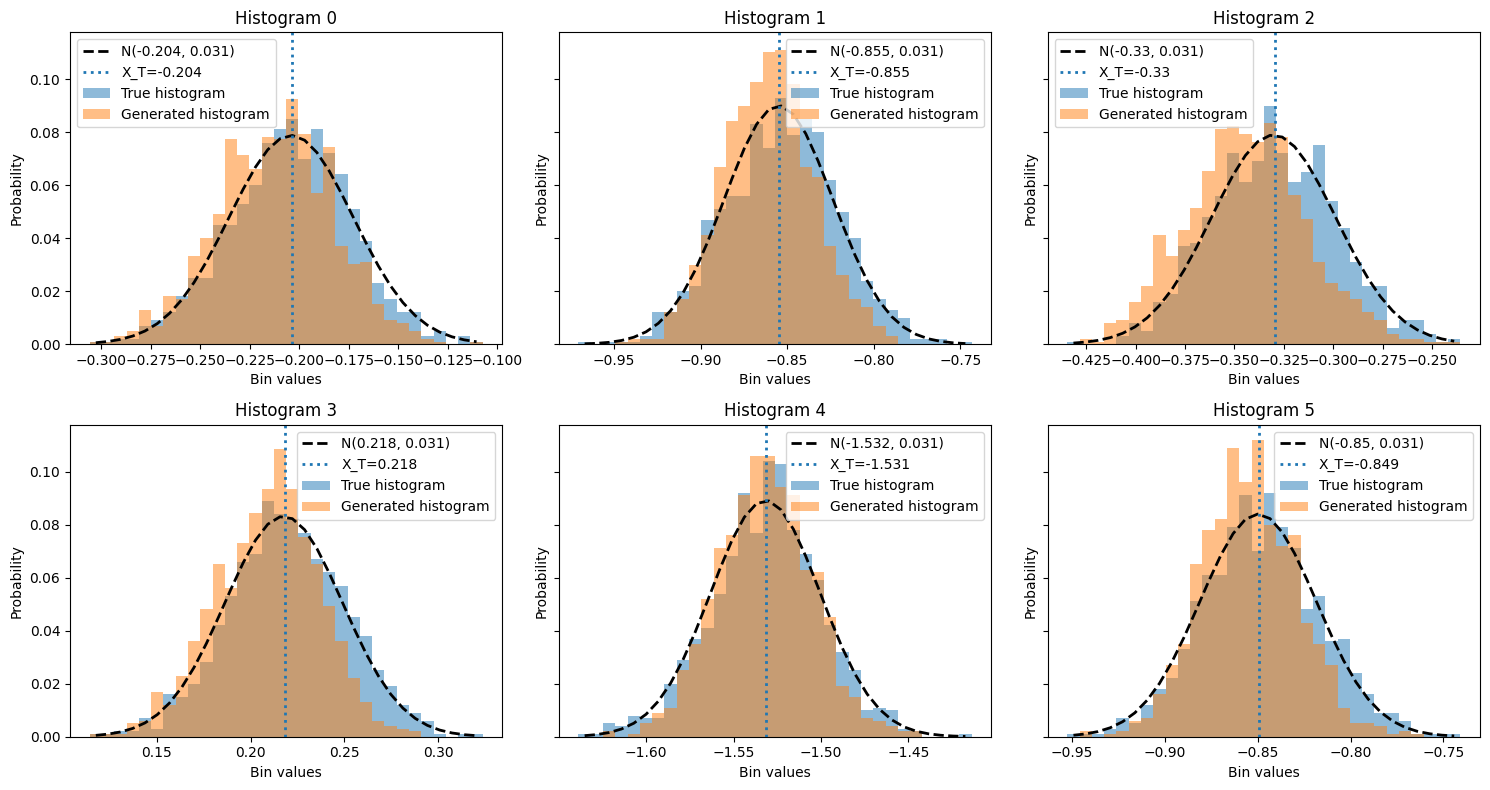
\includegraphics[width=1.0\textwidth]{Background/images/debug_forgan.png}
    \caption{Samples obtained using fixed $X_0$, $\mu$ and $\sigma = 0.5$.}
    \label{forgan_debug_sample}
\end{figure}


Also the results from the ForWGAN architecture with the same simplified setup are shown below:

\begin{table}[H] 
\centering
\caption{ForWGAN Architecture and Hyperparameters Summary}
\label{tab:forwgan_debug_architecture}
\begin{tabular}{lll}
\hline
\textbf{Parameter}         & \textbf{Generator}            & \textbf{Critic (Discriminator)} \\ \hline
Input Dimension            & 24 (Latent) + 2 (Cond.)       & 1 (Data) + 2 (Cond.)            \\
Hidden Layers              & [64, 128, 64]                 & [64, 128, 64, 32]               \\
Output Dimension           & 1                             & 1                               \\
Activation Function        & Leaky ReLU                    & Leaky ReLU                      \\
Normalization              & None                          & LayerNorm                      \\
Dropout                    & 0.0                           & 0.0                             \\
\multicolumn{3}{c}{\textbf{Global Training Settings}}                                     \\ \hline
Max Epochs                 & \multicolumn{2}{l}{100}                                       \\
\end{tabular}
\end{table}


\begin{table}[h]
\centering
\begin{tabular}{l c}
\hline
\textbf{Metric} & \textbf{Value} \\
\hline
\label{tab:forwgan_debug_results}
KS Test Acceptance (\%) & 1.0000 \\
JS Distance & 0.1493 \\
Hellinger Distance & 0.1301 \\
TV Distance & 0.1193 \\
EMD Distance & 0.0036 \\
\hline
\end{tabular}
\caption{Evaluation metrics rounded to four decimal places}
\end{table}


\begin{figure}[H]
    \centering
    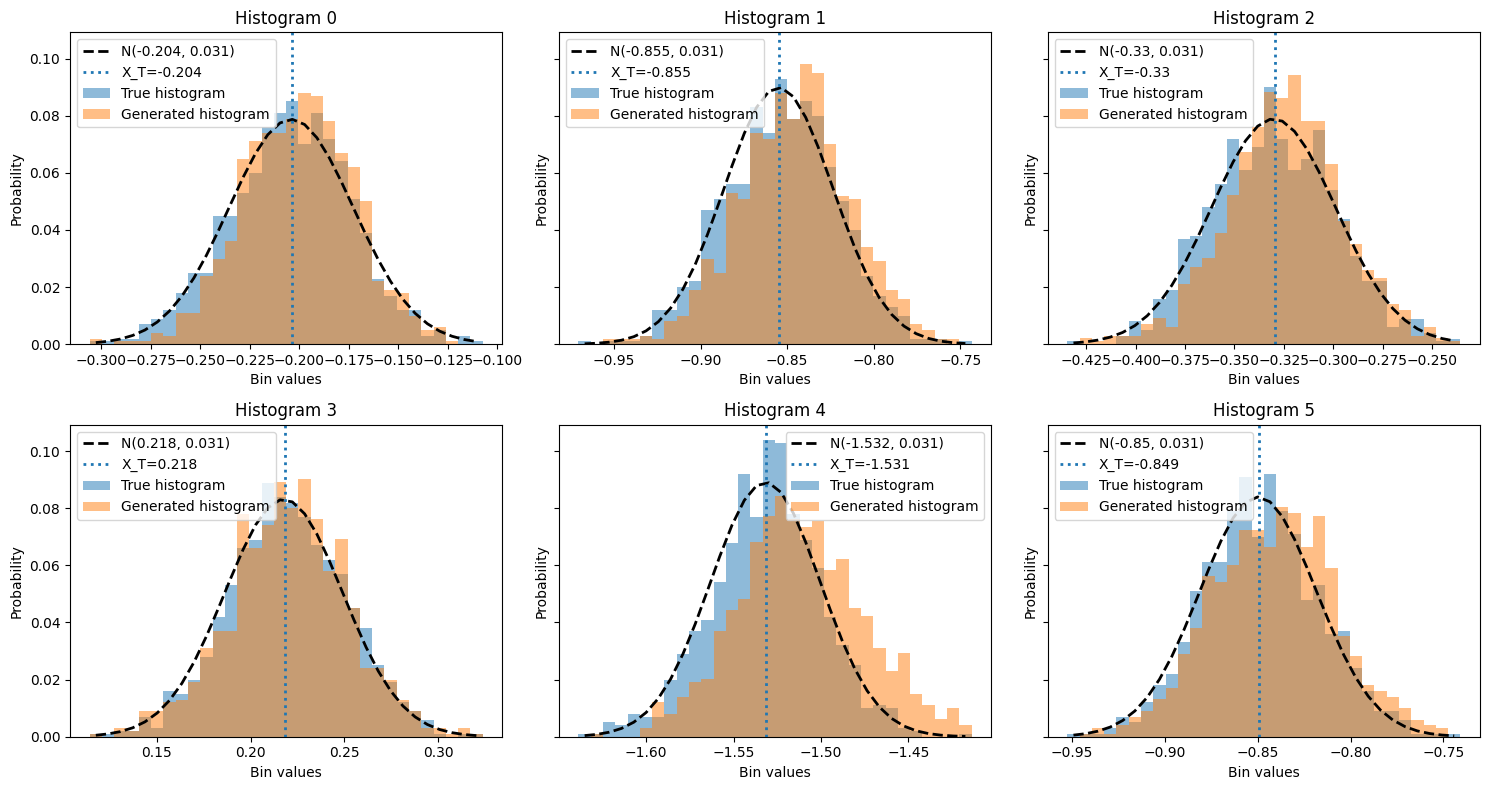
\includegraphics[width=1.0\textwidth]{Background/images/debug_forwgan.png}
    \caption{Samples obtained using fixed $X_0$, $\mu$ and $\sigma = 0.5$.}
    \label{forwgan_debug_sample}
\end{figure}

\subsection{ForGAN results}

The training algorithm and data flow used for training the ForGAN model shows just some changes related to the output and the way the probability distribution is generated.
In fact, in this case the output data of the training set is a single value $c_{T + \tau}$ instead of a probability vector as in the previous CGAN and CWGAN-GP models.\\


The experiment has been conducted by using the following architecture and hyperparameters:
\begin{table}[H]
\centering
\caption{ForGAN Architecture and Hyperparameters Summary}
\label{tab:forgan_summary}
\begin{tabular}{lll}
\hline
\textbf{Parameter}         & \textbf{Generator}          & \textbf{Critic (Discriminator)} \\ \hline
Input Dimension            & 64 (Latent) + 252 (Cond.)   & 1 (Data) + 252 (Cond.)          \\
Hidden Layers              & [512, 256, 128, 64]         & [512, 256, 256, 128, 64]        \\
Output Dimension           & 1                           & 1                               \\
Activation Function        & ReLU                        & Leaky ReLU                      \\
Normalization              & Batch Norm                  & None                      \\
Dropout                    & 0.0                         & 0.0                             \\
\multicolumn{3}{c}{\textbf{Global Training Settings}}                                     \\ \hline
Max Epochs                 & \multicolumn{2}{l}{100}                                       \\
\end{tabular}
\end{table}

The Kolmogorov-Smirnov test performed on 1000 real and generated bins probabilities shows that
the resulting p-values are accepted 48\% of times, which is inline with the results obtained for the CGAN model.\\
Moreover, the average Jenshen-Shannon divergence over the 1000 samples is around 0.49 which is worse than the CWGAN-GP model, suggesting that Wasserstein distance provides a better training convergence and generalization capabilities.

\begin{table}[h]
\centering
\begin{tabular}{l c}
\hline
\textbf{Metric} & \textbf{Value} \\
\hline
EMD Distance & 0.0255 \\
JS Distance & 0.4378 \\
Hellinger Distance & 0.4001 \\
TV Distance & 0.4129 \\
\hline
\end{tabular}
\caption{ForGAN performance metrics averaged over 1000 samples}
\end{table}

These results strongly suggest trying to improve the performances of the proposed ForGAN by adopting the Wasserstein distance instead of the BCE loss.\\
In order to visually assess the capabilities of the model,
different samples have been drawn such that every sampling parameter is fixed except for the volatility $\sigma$.
In particular, six different samples are shown below where
the starting values is the same $X_0 = 0.0$, $\mu = 0.0$ while the volatility have different values for each sample 
$\sigma = [0.3, 0.5, 0.7, 0.9]$. From the results can be notices that also this new architecture
struggles to effectively capture the variance of the target distribution when the volatility parameter is high.

\begin{figure}[H]
    \centering
    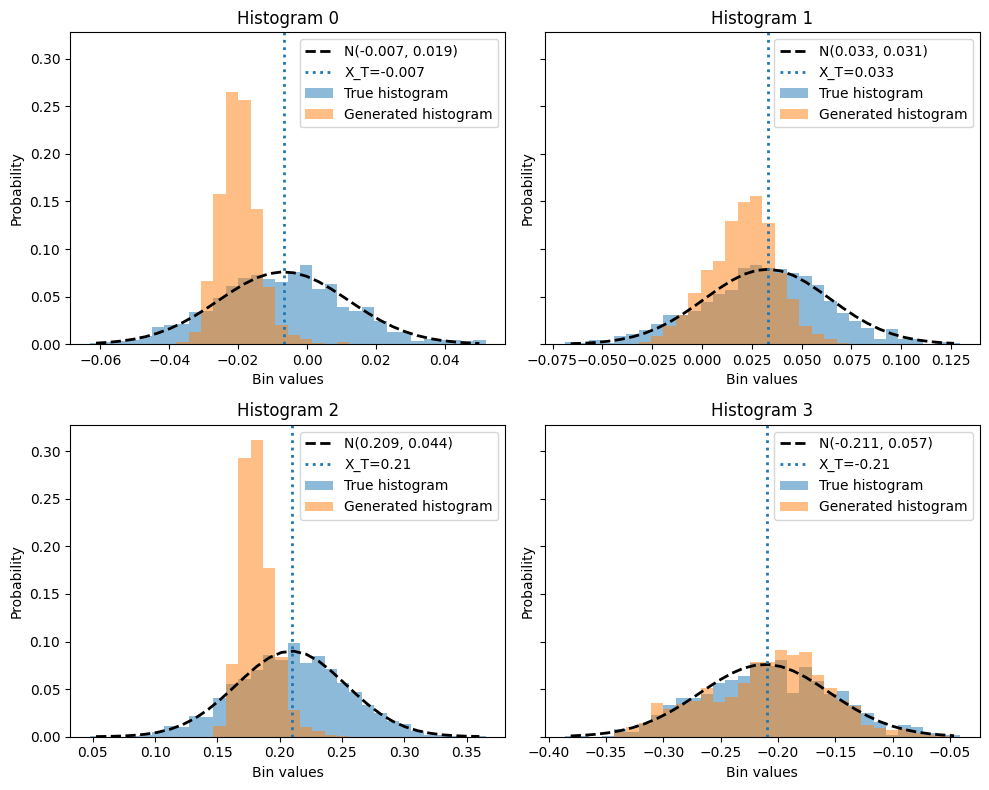
\includegraphics[width=1.0\textwidth]{Background/images/samples_forgan_simple.png}
    \caption{Samples obtained using fixed $X_0$ and $\mu$ while varying $\sigma = [0.3, 0.5, 0.7, 0.9]$.}
    \label{forgan_simple_sample_sigma}
\end{figure}



\subsection{ForWGAN results}
Also in this case the training algorithm and data flow used for training the ForWGAN model have been adapted to the new output setup.


The experiment has been conducted by using the following architecture and hyperparameters:
\begin{table}[H]
\centering
\caption{ForWGAN Architecture and Hyperparameters Summary}
\label{tab:forwgan_summary}
\begin{tabular}{lll}
\hline
\textbf{Parameter}         & \textbf{Generator}          & \textbf{Critic (Discriminator)} \\ \hline
Input Dimension            & 64 (Latent) + 252 (Cond.)   & 1 (Data) + 252 (Cond.)          \\
Hidden Layers              & [512, 256, 128, 64]         & [512, 256, 256, 128, 64]        \\
Output Dimension           & 1                           & 1                               \\
Activation Function        & ReLU                        & Leaky ReLU                      \\
Normalization              & None                        & Layer Norm                      \\
Dropout                    & 0.0                         & 0.0                             \\
\multicolumn{3}{c}{\textbf{Global Training Settings}}                                     \\ \hline
Max Epochs                 & \multicolumn{2}{l}{100}                                       \\
\end{tabular}
\end{table}


The Kolmogorov-Smirnov test performed on 1000 real and generated bins probabilities shows that
the resulting p-values are accepted 56\% of times, significantly higher than the CWGAN-GP and the ForGAN proposed models.\\
Moreover, the average Jenshen-Shannon divergence over the 1000 samples is around 0.35 which highlights an improvement with respect to the ForGAN model.\\
\begin{table}[h]
\centering
\begin{tabular}{l c}
\hline
\textbf{Metric} & \textbf{Value} \\
\hline
EMD distance & 0.0180 \\
JS Distance & 0.3402 \\
Hellinger Distance & 0.3110 \\
TV Distance & 0.3239 \\
\hline
\end{tabular}
\caption{ForWGAN performance metrics averaged over 1000 samples}
\end{table}


A visual inspection of different samples with various degrees of volatility is presented below
In particular, six different samples are shown below where
the starting values is the same $X_0 = 0.0$, $\mu = 0.0$ while the volatility have different values for each sample 
$\sigma = [0.3, 0.5, 0.7, 0.9]$.
From the results we can see an important improvement with respect to the simple ForGAN architecture 
in the same way as the CWGAN-GP model showed better results than the CGAN one,
suggesting that the Wasserstein loss with gradient penalty helps in stabilizing the training process and improving the quality of the generated distributions.

\begin{figure}[H]
    \centering
    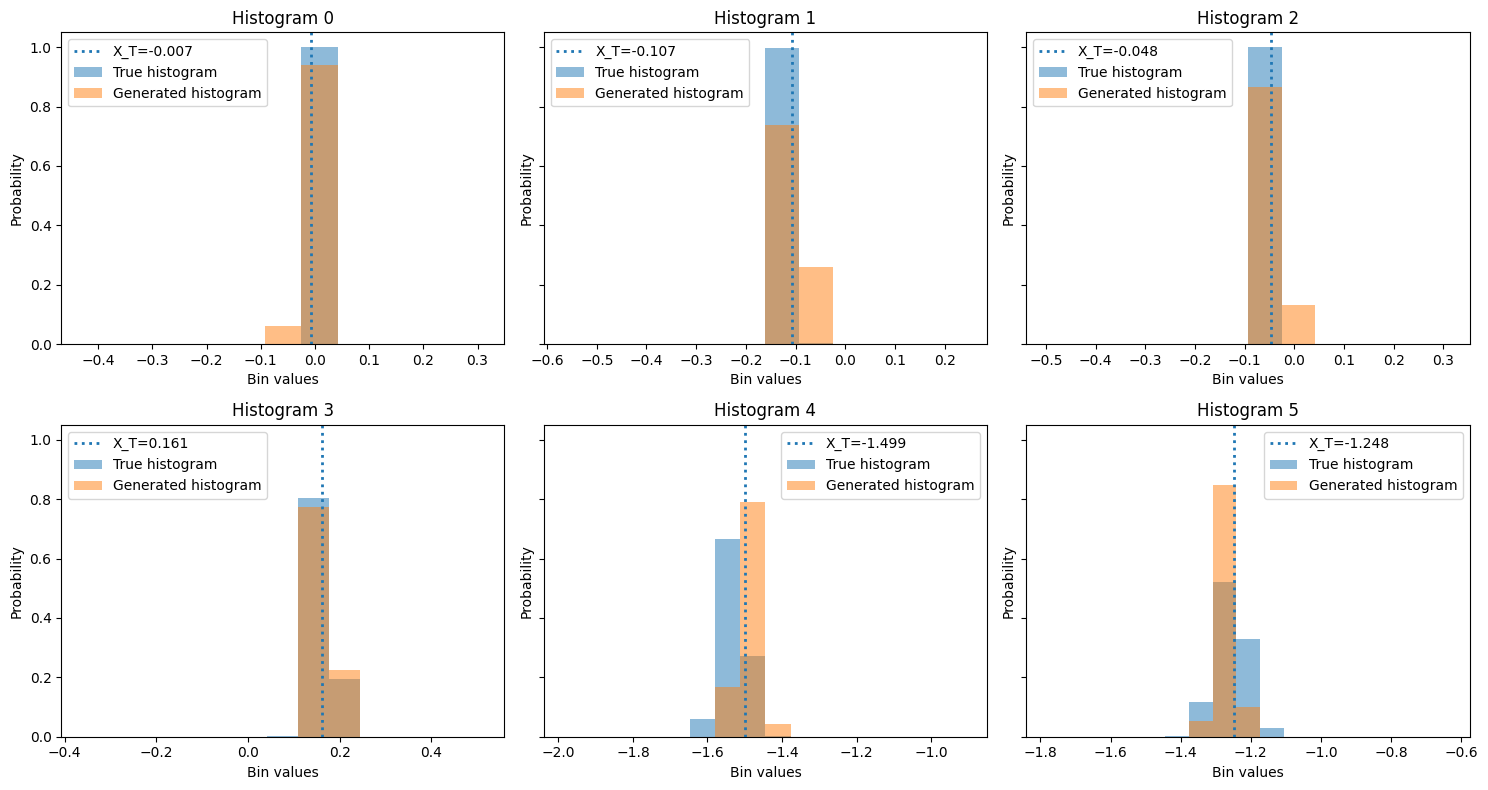
\includegraphics[width=1.0\textwidth]{Background/images/samples_forgan.png}
    \caption{Samples obtained using fixed $X_0$ and $\mu$ while varying $\sigma = [0.3, 0.5, 0.7, 0.9]$.}
    \label{forgan_sample_sigma}
\end{figure}



\subsection{Improvements}
Mode collapse, also known as the "Helvetica scenario," 
occurs when the generator learns to produce only a 
limited subset of the data distribution. 
It can be categorized into two forms, especially in the context of 
conditional time-series GANs like ForGAN:
\begin{itemize}
    \item Distribution Mode Collapse: A collapse in the variety of samples generated for a single specific condition (time point). The model fails to capture the probabilistic uncertainty of the future return.
    \item Mean Mode Collapse: A collapse in the distribution of the means of generated values across all different conditions. This effectively reduces the model to producing similar point estimates regardless of the historical input
\end{itemize}

When both occur simultaneously, 
the model yields a single point estimate for every input, 
completely losing its probabilistic forecasting capabilities. 
Research indicates that mode collapse is often tied to the generator converging toward sharp local minima. 
Once $G$ finds a sample that receives a high score from $D$, it may continue to reproduce that sample; 
if $D$ cannot identify this repetitive behavior (due to converging to its own local minima), 
the gradients for $G$ vanish, and the model becomes stuck.\\

